\documentclass[]{article}
\usepackage{lmodern}
\usepackage{amssymb,amsmath}
\usepackage{ifxetex,ifluatex}
\usepackage{fixltx2e} % provides \textsubscript
\ifnum 0\ifxetex 1\fi\ifluatex 1\fi=0 % if pdftex
  \usepackage[T1]{fontenc}
  \usepackage[utf8]{inputenc}
\else % if luatex or xelatex
  \ifxetex
    \usepackage{mathspec}
  \else
    \usepackage{fontspec}
  \fi
  \defaultfontfeatures{Ligatures=TeX,Scale=MatchLowercase}
\fi
% use upquote if available, for straight quotes in verbatim environments
\IfFileExists{upquote.sty}{\usepackage{upquote}}{}
% use microtype if available
\IfFileExists{microtype.sty}{%
\usepackage{microtype}
\UseMicrotypeSet[protrusion]{basicmath} % disable protrusion for tt fonts
}{}
\usepackage[margin=1in]{geometry}
\usepackage{hyperref}
\hypersetup{unicode=true,
            pdftitle={Spherelets},
            pdfauthor={Caleb Ren},
            pdfborder={0 0 0},
            breaklinks=true}
\urlstyle{same}  % don't use monospace font for urls
\usepackage{graphicx,grffile}
\makeatletter
\def\maxwidth{\ifdim\Gin@nat@width>\linewidth\linewidth\else\Gin@nat@width\fi}
\def\maxheight{\ifdim\Gin@nat@height>\textheight\textheight\else\Gin@nat@height\fi}
\makeatother
% Scale images if necessary, so that they will not overflow the page
% margins by default, and it is still possible to overwrite the defaults
% using explicit options in \includegraphics[width, height, ...]{}
\setkeys{Gin}{width=\maxwidth,height=\maxheight,keepaspectratio}
\IfFileExists{parskip.sty}{%
\usepackage{parskip}
}{% else
\setlength{\parindent}{0pt}
\setlength{\parskip}{6pt plus 2pt minus 1pt}
}
\setlength{\emergencystretch}{3em}  % prevent overfull lines
\providecommand{\tightlist}{%
  \setlength{\itemsep}{0pt}\setlength{\parskip}{0pt}}
\setcounter{secnumdepth}{5}
% Redefines (sub)paragraphs to behave more like sections
\ifx\paragraph\undefined\else
\let\oldparagraph\paragraph
\renewcommand{\paragraph}[1]{\oldparagraph{#1}\mbox{}}
\fi
\ifx\subparagraph\undefined\else
\let\oldsubparagraph\subparagraph
\renewcommand{\subparagraph}[1]{\oldsubparagraph{#1}\mbox{}}
\fi

%%% Use protect on footnotes to avoid problems with footnotes in titles
\let\rmarkdownfootnote\footnote%
\def\footnote{\protect\rmarkdownfootnote}

%%% Change title format to be more compact
\usepackage{titling}

% Create subtitle command for use in maketitle
\newcommand{\subtitle}[1]{
  \posttitle{
    \begin{center}\large#1\end{center}
    }
}

\setlength{\droptitle}{-2em}

  \title{Spherelets}
    \pretitle{\vspace{\droptitle}\centering\huge}
  \posttitle{\par}
  \subtitle{Stat 185 Term Paper}
  \author{Caleb Ren}
    \preauthor{\centering\large\emph}
  \postauthor{\par}
      \predate{\centering\large\emph}
  \postdate{\par}
    \date{December 14, 2019}

\usepackage{algorithm}
\usepackage{algorithmic}
\usepackage{booktabs}
\usepackage{longtable}
\usepackage{array}
\usepackage{multirow}
\usepackage{wrapfig}
\usepackage{float}
\usepackage{colortbl}
\usepackage{pdflscape}
\usepackage{tabu}
\usepackage{threeparttable}
\usepackage{threeparttablex}
\usepackage[normalem]{ulem}
\usepackage{makecell}
\usepackage{xcolor}

\begin{document}
\maketitle

{
\setcounter{tocdepth}{2}
\tableofcontents
}
\newpage

\section{Introduction}

Data that exists in a high-dimensional ambient space may instead be
considered to lie near a lower dimensional manifold (e.g.~a circle in
\(\mathbb{R}^2\) that lies ambiently in \(\mathbb{R}^3\) space). Many
techniques are focused on reducing the ambient space to one closer to
the intrinsic space such as clustering (Duda, Stork, and Hart 2000),
data compression (Hurtado 2012), and predictive modelling (Lee and
Verleysen 2008). Many of these techniques that attempt to approximate
manifolds embedded in a lower dimensional space are locally linear, use
multiscale dictionaries, and as such struggle with areas with high
Gaussian curvature. Additionally, many techniques that approximate local
manifolds do not perform well with out-of-sample error as they do not
reveal much information on the traits of the lower dimension manifold.

A simple alternative that is able to handle curvature as well as
out-of-sample error is to use pieces of (hyper)spheres to locally
approximate the unknown subspace (Didong Li and Dunson 2019). This
method was first proposed by Li and Dunson, who termed the technique
spherical PCA (SPCA) (Li and Dunson 2017), or \emph{spherelets} for
short. Whereas principal component analysis (PCA) is an
eigenvalue/eigenvector problem from an inherently \emph{linear}
dimension reduction problem, spherelets rely on projection mappings to
the surfaces of a hypersphere as an underlying mechanism. As such, in
simple cases of SPCA, closed form analytic solutions exist and can be
seen as a generalization of PCA that is able to incorporate degrees of
curvature. Spherical PCA in general does not have a closed-form solution
due to the myriad ways in which a particular dataset can be partitioned
and fit with sub-manifolds. Various algorithms exist to best partition
the original dataset such as cover trees (Beygelzimer, Kakade, and
Langford 2006), METIS (Karypis and Kumar 1998), and iterated PCA (Szlam
2009). The type of partitioning done is context-dependent and multiple
types of subsetting can be done to cross-validated to reduce test MSE.
As examples, we will examine two types of partitioning: naively---by
splitting the dataset into equal-sized clusters---and via partioning by
iterated PCA (Didong Li and Dunson 2019).

Data that is represented in higher dimension \(\mathbb{R}^D\) can be
projected down to a manifold in \(\mathbb{R}^d\) consisting of a set of
spherelets in \(\mathbb{R}^d\). Ultimately, the algorithm partitions the
dataset into \(k\) subsets, each of which is fit with a submanifold
\(M_k \in \mathbb{R}^d\) with a corresponding projection map
\(\Psi_k: \mathbb{R}^D \rightarrow \mathbb{R}^d\). Given a dataset
\(\mathbf{X} \in \mathbb{R}^D\), the spherical PCA algorithm returns
manifold \(M\) and the projection map \(\Psi\), which are the manifold
and mapping from the data to the approximate manifold in
\(\mathbb{R}^d\), respectively.

Manifold approximation for model-building is one useful application of
spherelets but the technique can be used for other purposes. Spherical
PCA can also be used to denoise manifolds and generate visualizations of
data in higher dimensions. Spherelets have been shown to outperform
competiting denoising algorithms like Gaussian Blurring Mean Shift
(GBMS), Manifold Blurring Mean Shift (MBMS), and Local Tangent
Projection (LTP). Visualization techniques that preserve local geometry
like Isomap, Locally Linear Embedding (LLE), and t-distributed
Stochastic Neighborhood Embedding (t-SNE) can also be modified to
incorporate spherical geometry using the same projection to spherical
affine subspace, as in the original spherelets paper (Didong Li and
Dunson 2019).

In spherical PCA, a point \(\vec{y}_i\) is projected down to a sphere
\(S_V(c, r)\), where \(c\) is the center of the sphere, \(r\) is the
radius, and \(V\) specifies the subspace on which the sphere lies. The
optimal estimates for the sphere \(S_{\hat{V}}(\hat{c}, \hat{r})\) are
given by:

\[
\begin{gathered}
\hat{V} = (\vec{v}_1, \dots, \vec{v}_{d + 1}) \\
\hat{c} = -\frac{\vec{\eta}^\star}{2}  \\
\hat{r} = \frac{1}{N} \sum_{k = 1}^N \left\|\vec{z}_i - \hat{c} \right\|
\end{gathered}
\]

Where \(\vec{v}_i\) is the \(i\)th eigenvector of the covariance matrix
times \(\mathbf{\Sigma}\), \(\vec{z}_i\) is the the projected data down
to the subspace and \(\vec{\eta}^\star\) is a vector based on the entire
projected dataset \(\mathbf{Z}\). After an introduction into notation of
spherical PCA, I will introduce relevant theory, including the Main
Theorem that undergirds spherical PCA. Assumptions made in spherical PCA
are covered in section \_\_\_\_\_\_ and I will provide numerical
examples demonstrating areas in which spherelets perform well and poorly
based on the intrinsic structure of the manifold in Section 4.

\section{Method}

\subsection{Notation}

Assume we have the \(N \times D\) data matrix \(\mathbf{X}\), with \(N\)
observations and \(D\) variable where \(x_{i,j}\) represents the \(i\)th
observation of the \(j\)th variable:

\[
\mathbf{X} = \begin{bmatrix}
x_{1,1} & \dots & x_{1,D} \\
\vdots & \ddots & \vdots \\
x_{i,1} & \dots & x_{i,D} \\
\vdots & \ddots & \vdots \\
x_{N,1} & \dots & x_{N,D}
\end{bmatrix}
\]

As in linear PCA, a more succinct way to represent this matrix is to
write:

\[
\mathbf{X} = \begin{bmatrix} \vec{x}_1^T \\ \vdots \\ \vec{x}_i
^T\\ \vdots \\ \vec{x}_N^T \end{bmatrix}
\]

We will once again treat \(\vec{x}_1, \dots, \vec{x}_N\) as i.i.d.
samples of a random vector in \(\mathbb{R}^D\) from the same underlying
distribution \(F\) for which \(E_{x \sim F} \|x\|^2 < \infty\) to assure
that the mean and covariance of the data matrix are well-deefined. We
use:

\[
\overline{x} = \frac{1}{N} \sum_{i = 1}^N \vec{x}_i
\]

to denote the sample mean of \(\vec{x}\). To denote the covariance
operator, we use:

\[
\mathbf{\Sigma}_x = \frac{1}{N} \sum_{i = 1}^N (\vec{x}_i - \overline{x})(\vec{x}_i - \overline{x})^T = \frac{1}{N} \left(\sum_{i = 1}^N \vec{x}_i \vec{x}_i^T \right) - \overline{x}\overline{x}^T = \frac{1}{N} \mathbf{X}^T \mathbf{X} - \overline{x} \overline{x}^T
\]

This covariance operator will come into use later on. Additional
notation includes:

\begin{itemize}
\item
  \(1_N\) is the column vector of all ones with length \(N\) (i.e.
  \(1_N \in \mathbb{R}^N\))
\item
  \(\| \vec{z} \|\) denotes the Euclidean norm (i.e.~for
  \(\vec{z} \in \mathbb{R}^d, \|\vec{z}\| = \left(\sum_{i = 1}^{d} z_i ^2 \right)^{1/2} = \sqrt{\vec{z}^T \vec{z}}\))
\item
  \(\Psi: \mathbb{R}^D \rightarrow \mathbb{R}^{d+1}\) is a projection
  map from space \(\mathbb{R}^D\) to \(\mathbb{R}^{d+1}\). Note:
  \(\Psi\) maps from \(\mathbb{R}^D\) to \(\mathbb{R}^{d+1}\) rather
  than \(\mathbb{R}^{d}\) because the projected points lie on an affine
  subspace with one fewer degree of freedom than the manifold. One
  example is fitting a curve in \(\mathbf{R}^2\) with sections of
  2-dimensional circles; while circles are 2D, the projected points only
  live along the edge of the circle. As such, we include on extra
  dimension in our projection map to account for the extra degree of
  freedom.
\item
  \(d^2(\cdot, \cdot)\) is the distance operator between two points.
  Note that \(d^2(x, y)\) is equivalent to \(\sqrt(\| x - y \|)\).
\end{itemize}

\subsection{Main Theorem}

The Main Theorem underlying spherical PCA describes the

\subsection{Spherical PCA}

Given a set of data \(\vec{x}_1, \dots, \vec{x}_N \in \mathbb{R}^D\), we
find the best approximating sphere \(S_{V}(c,r)\), where \(c\) is the
center, \(r\) is the radius, and
\(V \in \mathbb{R}^{(d+1) \times (d+1)}\) is the \((d+1)\)th dimensional
affine subspace the sphere lives on. For any point in the dataset
\(\vec{x}_i\), the closest point \(\vec{y}_i\) lying on the sphere
\(S_V(c,r)\) is the point that minimizes Euclidean distance
\(\|x,y\|^2\) between \(x\) and \(y\). The optimal subspace \(V\) is
given by \(\hat{V} = (\vec{v}_1, \dots, \vec{v}_{d+1})\), where
\(\vec{v}_i, i \in \{1,\dots,d+1\}\) is the \(i\)th eigenvector ranked
in descending order of
\((\mathbf{X} - 1_N\bar{\mathbf{X}})^T(\mathbf{X} - 1_N\bar{\mathbf{X}})\).

If
\(\vec{z}_i = \bar{\mathbf{X}} + \hat{V}\hat{V}^T(\vec{x}_i - \bar{\mathbf{X}})\)
are a change of basis to affine subspace \(V\), then it can be shown
that the minimizing pair \((\vec{\eta}^\star, \vec{\xi}^\star)\) of loss
function
\(g(\vec{\eta}, \vec{\xi}) = \sum_{k = 1}^N(\vec{z}_i^T \vec{z}_i + \vec{\eta}^T \vec{x}_i + \vec{\xi})^2\)
is:

\[
\begin{gathered}
\vec{\eta} = -H^{-1}\omega \\
\vec{\xi} = -\frac{1}{N} \sum_{k=1}^N(\vec{z}_i^T \vec{z}_i + \vec{\eta}^T\vec{z}_i)
\end{gathered}
\]

where \(H\) and \(\omega\) are defined as:

\[
\begin{gathered}
H = \sum_{k = 1}^N (\vec{z}_i - \overline{z})(\vec{z}_i - \vec{z})^T \\
\vec{\omega} = \sum_{k=1}^N \left( \|\vec{z}_i^T\vec{z}_i\| - \frac{1}{N}\sum_{j=1}^N\|\vec{z}_j^T\vec{z}_j\| \right) (\vec{z}_i - \overline{z})
\end{gathered}
\]

The optimal parametrization \((\hat{V}, \hat{c}, \hat{r})\) of the
projection of \(\mathbf{X} \in \mathbb{R}^{N \times D}\) onto the sphere
\(S_V(c, r)\) is:

\[
\begin{gathered}
\hat{V} = (\vec{v}_1, \dots, \vec{v}_{d + 1}) \\
\hat{c} = -\frac{\vec{\eta}^\star}{2}  \\
\hat{r} = \frac{1}{N} \sum_{k = 1}^N \left\|\vec{z}_i - \hat{c} \right\|
\end{gathered}
\]

The projection map \(\hat{\Psi}\) of data matrix \(\mathbf{X}\) onto
sphere \(S_{\hat{V}}(\hat{c}, \hat{r})\) is the projection map onto
affine subspace \(\hat{c} + \hat{V}\), given by:

\[
\hat{\Psi}(\vec{x}_i) = \hat{c} + \frac{\hat{r}}{\| \hat{V}\hat{V}^T (\vec{x}_i - \hat{c}) \|}\hat{V}\hat{V}^T(\vec{x}_i - \hat{c})
\]

\subsection{Local SPCA}

We have now defined spherical PCA (SPCA) to project the data
\(\mathbf{X}\) down to single sphere \(S_V\). However, this single
sphere will typically not be a sufficient approximation for the inherent
manifold \(M\). Instead, we partition the space \(\mathbb{R}^D\) into
\(k\) disjoint subsets \(C_1, \dots, C_k\). For the \(k\)th disjoint
subset, we can define a data matrix
\(\mathbf{X}_k = \{X_i : X_i \in C_k\}\) that is a partition of the
original data that lies within \(C_k\). After applying SPCA to
\(\mathbf{X}_k\), we obtain spherical volume, center, and radius
\((\hat{V}_k, \hat{c}_k, \hat{r}_k)\) alongside projection map
\(\Phi_k\) as a map from \(x\in C_k\) to
\(y \in S_{\hat{V}_k}(\hat{c}_k, \hat{r}_k)\). A spherelets estimation
\(\hat{M}\) of the manifold \(M\) can be obtained by setting
\(\hat{M} = \bigcup_{k = 1}^K \hat{M}_k\), where \(\hat{M}_k\) is the
local SPCA in the \(k\)th region and
\(\hat{M}_k = S_{\hat{V}_k}(\hat{c}_k, \hat{r}_k) \cap C_k\)

\subsection{Assumptions}

There are two main

\subsection{Method}

The algorithm is as follows:

\begin{algorithm}[H]
  \caption{Spherelets}
  \textbf{Input:} Data matrix $\mathbf{X}$; intrinsic dimension $d$; partition $\{C_k\}_{k = 1}^K$ \\
  \textbf{Output:} Local estimated manifolds $\hat{M}_k$ and projection map $\hat{\Psi}_k, k \in \{1, \dots, K\}$; global estimated manifold $\hat{M}$ of intrinsic manifold $M$ and projection map $\hat{\Psi}$
  \begin{algorithmic}[1]
    \FOR{(k = 1 : K)}
      \STATE Define $\mathbf{X}_{[k]} = \mathbf{X} \cap C_k$\; \\
      \STATE Calculate $\hat{V}_k, \hat{c}_k, \hat{r}_k$\; \\
      \STATE Calculate $\hat{\Psi}_k(x) = \hat{c}_k + \frac{\hat{r}_k}{\|\hat{V}_k\hat{V}_k^T(x-\hat{c}_k)\|}(x - \hat{c}_k)$\; \\
      \STATE Calculate $\hat{M}_k = S_{\hat{V}_k}(\hat{c}_k, \hat{r}_k) \cap C_k$\;
    \ENDFOR
    \STATE Calculate $\hat{\Psi}(x) = \sum_{k = 1}^K \mathbf{1}_{\{x \in C_k\}}\hat{\Psi}_k(x)$, and $\hat{M} = \bigcup_{k =1}^K\hat{M}_k$.
  \end{algorithmic}
\end{algorithm}

\section{Strengths and Weaknesses}

\subsection{Strengths}

\begin{itemize}
\tightlist
\item
  Performs well in areas with high curvature that local PCA can't
  approximate
\item
  Can perform OOS assessments and returns the underlying manifold
\end{itemize}

\subsection{Weaknesses}

\begin{itemize}
\tightlist
\item
  Struggles with areas of non-uniform curvature
\item
  Struggles with non-uniform dimensions
\item
  Must specify inherent dimension \(d\)
\item
  Computationally expensive
\item
  Dependent on choice of manifold subsetting
\end{itemize}

\section{Examples}

To generate numerical examples, I used the \texttt{SPCA} and
\texttt{SS\_calc} functions written by co-author Minerva Mukhopadhyay
(mmukhopadhyay 2019). The \texttt{SPCA} function takes in a matrix of
\(N\) observations \(\vec{x}_i \in \mathbb{R}^{D}, i \in 1, \dots, N\)
and returns the error given by spherical and local PCA (\texttt{SS} and
\texttt{SS\_new}), as well as the projected values \texttt{Y\_D}.

\subsection{Euler Spiral}

The Euler spiral is a curve in \(\mathbb{R}^1\) that has a curvature
that changes linearly with arc length. In other words,
\(\kappa(s) = s\). The Euler spiral can be parametrized as follows:

\[
\begin{bmatrix}x(s) \\ y(s)\end{bmatrix} = 
\begin{bmatrix}
\displaystyle\int_0^s \cos(t^2) dt \\
\displaystyle\int_0^s \sin(t^2) dt
\end{bmatrix} \hspace{0.1in} s \in [0, 4]
\]

We use the Euler spiral as a demonstration to see how spherical PCA is
able to handle regions with curvature.

\begin{center}\includegraphics{Term_paper_files/figure-latex/Euler-1} \end{center}

\begin{figure}[H]

{\centering 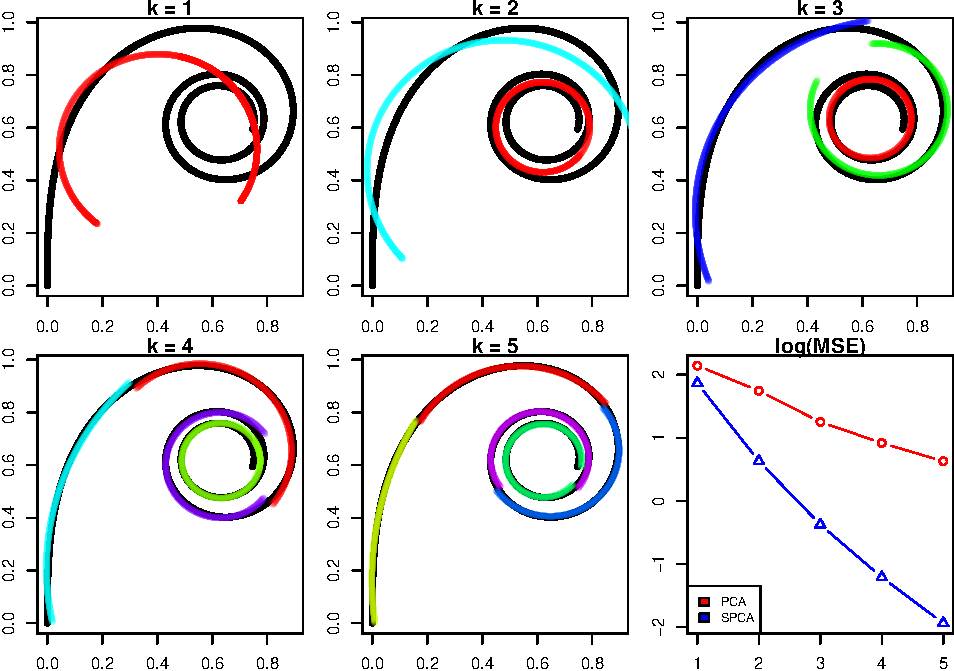
\includegraphics{Term_paper_files/figure-latex/euler-1} 

}

\caption{Spherical PCA performed on an Euler spiral with $k = 3, 8$.}\label{fig:euler}
\end{figure}

\subsection{Helix}

\begin{figure}[H]

{\centering 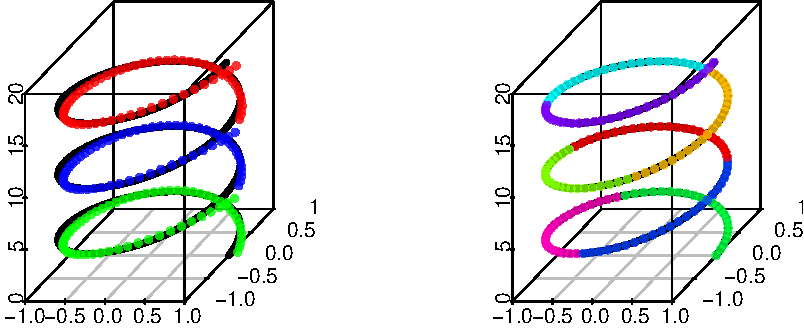
\includegraphics{Term_paper_files/figure-latex/helix-1} 

}

\caption{Spherical PCA performed on a helix with $k = 3, 8$.}\label{fig:helix}
\end{figure}

\subsection{Cylinder}

\begin{verbatim}
## [1] 0.00269493
\end{verbatim}

\begin{verbatim}
## [1] 7.353559e-05
\end{verbatim}

\begin{figure}[H]

{\centering 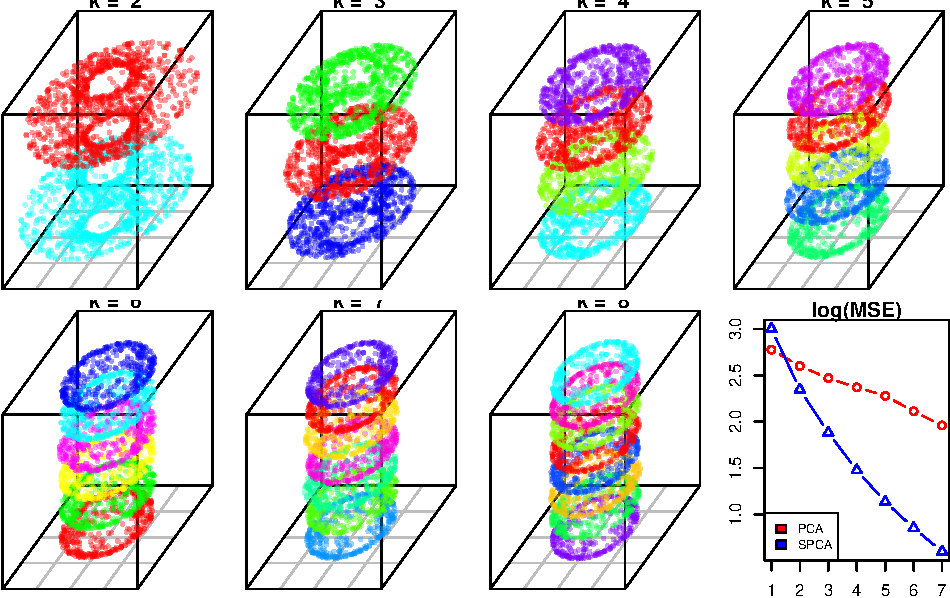
\includegraphics{Term_paper_files/figure-latex/cylinder-1} 

}

\caption{Spherical PCA performed on a cylinder with $k = 3, 8$.}\label{fig:cylinder}
\end{figure}

We see that SPCA is not fully capable of handling a cylinder.

\newpage

\section{References}

\hypertarget{refs}{}
\hypertarget{ref-beygelzimer2006}{}
Beygelzimer, Alina, Sham Kakade, and John Langford. 2006. ``Cover Trees
for Nearest Neighbor.'' ACM.

\hypertarget{ref-li2019}{}
Didong Li, Minerva Mukhopadhyay, and David B Dunson. 2019. ``Efficient
Manifold Approximation with Spherelets.'' \emph{arXiv}, February.

\hypertarget{ref-duda2000}{}
Duda, Richard O, David G Stork, and Peter E Hart. 2000. \emph{Pattern
Classification}. 2nd ed. Wiley.

\hypertarget{ref-hurtado2012}{}
Hurtado, Jorge E. 2012. \emph{Structural Reliability}. Vol. 17.
Springer-Verlag.

\hypertarget{ref-karypis1998}{}
Karypis, George, and Vipin Kumar. 1998. ``A Fast and High Quality
Multilevel Scheme for Partitioning Irregular Graphs.'' \emph{SIAM
Journal on Scientific Computing} 20 (1): 359--92.
doi:\href{https://doi.org/10.1137/s1064827595287997}{10.1137/s1064827595287997}.

\hypertarget{ref-lee2008}{}
Lee, John A, and Michel Verleysen. 2008. \emph{Nonlinear Dimensionality
Reduction}. Springer Science.

\hypertarget{ref-li2017}{}
Li, Didong, and David B Dunson. 2017. ``Efficient Manifold and Subspace
Approximations with Spherelets.'' \emph{arXiv}, June. ResearchGate.

\hypertarget{ref-github}{}
mmukhopadhyay. 2019. ``Efficient Manifold Learning Using Spherelets.''
Github. April 9.

\hypertarget{ref-szlam2009}{}
Szlam, Arthur. 2009. ``Asymptotic regularity of subdivisions of
Euclidean domains by iterated PCA and iterated 2-means.'' \emph{Applied
and Computational Harmonic Analysis}, March. Academic Press.
\url{https://www.sciencedirect.com/science/article/pii/S1063520309000190}.


\end{document}
